\section{Simulation results}
\label{sec:sim_res}

The program saves the simulation results in the \texttt{./results} subdirectory.

\subsection{Summary}
The summary is written to the \texttt{summary.csv} file, with the following columns: $day$ (zero-based), $country$, $susceptible$, $infected$ and $immune$.
At the end of each simulated day, the program writes a summary entry for each of the countries, so $(day, country)$ can be considered as a compound index.

\subsection{Trace}
By running the program with the \verb!--write-trace! option, each process will write a \texttt{trace\_\{country\}.csv} file on its local filesystem. It contains the attributes of each individual in that country at each time step.
After gathering these files in a single \texttt{results} directory, one can produce an animated representation of the simulation with the script \texttt{tools/trace\_animation.py}; the parameters at the end of the script must be changed to those of the performed simulation.

\begin{figure}[hb]
    \begin{subfigure}[c]{0.49\textwidth}
        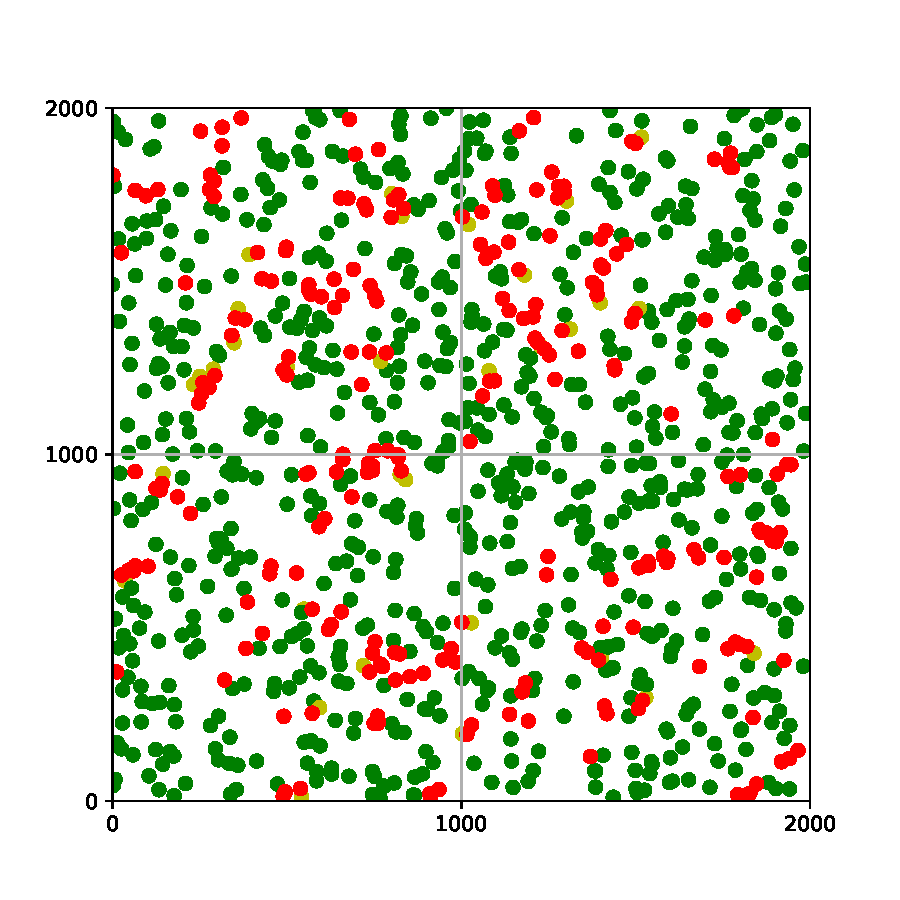
\includegraphics[width=\textwidth]{anim_f_50}
    \end{subfigure}
    ~
    \begin{subfigure}[c]{0.49\textwidth}
        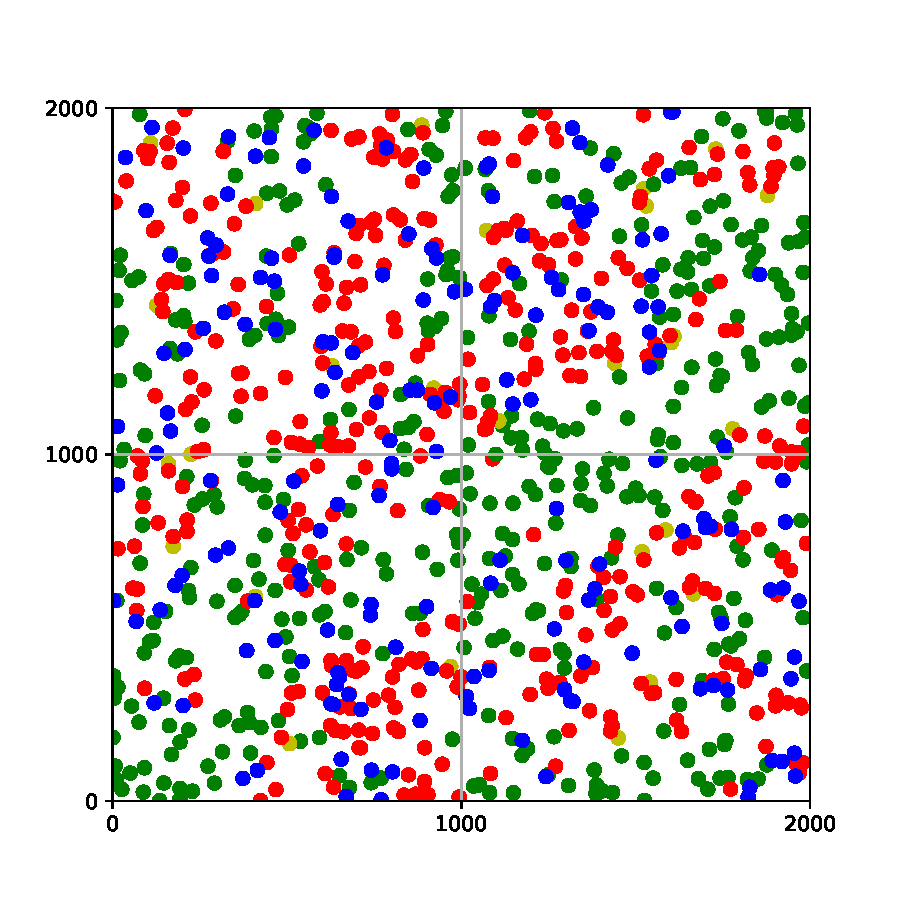
\includegraphics[width=\textwidth]{anim_f_150}
    \end{subfigure}
    \caption{Stills from an animation with 1000 individuals over 4 countries at $t=\SI{50}{s}$ and $t=\SI{150}{s}$. Color represents status:
    \textcolor{plt:green}{\circmark}~not~exposed,
    \textcolor{plt:yellow}{\circmark}~exposed,
    \textcolor{plt:red}{\circmark}~infected,
    \textcolor{plt:blue}{\circmark}~immune.
    }
    \label{fig:animation}
\end{figure}